\documentclass[11pt, oneside]{article}   	% use "amsart" instead of "article" for AMSLaTeX format
\usepackage{geometry}                		% See geometry.pdf to learn the layout options. There are lots.
\geometry{letterpaper}                   		% ... or a4paper or a5paper or ... 
%\geometry{landscape}                		% Activate for rotated page geometry
%\usepackage[parfill]{parskip}    		% Activate to begin paragraphs with an empty line rather than an indent
\usepackage{graphicx}				% Use pdf, png, jpg, or eps§ with pdflatex; use eps in DVI mode
								% TeX will automatically convert eps --> pdf in pdflatex		
\usepackage{amssymb}
\usepackage{amsmath}
\usepackage{braket}
\usepackage{siunitx}
\usepackage{mathtools}
%\usepackage{tensor}
%SetFonts

%SetFonts


\title{CIS state preparation on quantum circuit}
% Hardware efficient generation of a few particle states based on matrix product state
\author{Takahiro Yamamoto}
%\date{}							% Activate to display a given date or no date
\begin{document}

\maketitle

\subsection{Pauli rotation}
\begin{align}
R_x(\theta) &= e^{-i \theta X/2} = 
\begin{bmatrix}
\cos(\theta/2) & -i \sin(\theta/2) \\
-i \sin(\theta/2) & \cos(\theta/2)
\end{bmatrix} \\
R_y(\theta) &= e^{-i \theta Y/2} = 
\begin{bmatrix}
\cos(\theta/2) & -\sin(\theta/2) \\
\sin(\theta/2) & \cos(\theta/2)
\end{bmatrix} \\
R_z(\theta) &= e^{-i \theta Z/2} = 
\begin{bmatrix}
e^{-i \theta/2} & 0 \\
0 & e^{i \theta/2}
\end{bmatrix}
\end{align}

\section{CIS and circuit}
\subsection{Single-reference CI wave functions}
The FCI wave function is often dominated by a single reference configuration, usually the Hartree-Fock state.
It is then convenient to think of the FCI wave function as generated from this reference configuration by the application of a linear combination of spin-orbital excitation operators

\begin{equation}
\ket{\text{FCI}} = \left( 1 + \sum_{AI} \hat{X}^A_I + \sum_{A>B, I>J} \hat{X}^{AB}_{IJ} \right) \ket{\text{HF}} 
\end{equation}
where, for example,
\begin{align}
\hat{X}^A_I \ket{\text{HF}} &= C^A_I a^{\dagger}_A a_I \ket{\text{HF}} \\
\hat{X}^{AB}_{IJ} \ket{\text{HF}} &= C^{AB}_{IJ} a^{\dagger}_A a^{\dagger}_B a_I a_J \ket{\text{HF}} 
\end{align}

Thus, we may characterize the determinants in the FCI expansion as single (S), double (D), triple (T), quadruple (Q), and higher excitation relative to the Hartree-Fock state.

\subsection{CIS}
\begin{equation}
\ket{\text{FCI}} = \left( 1 + \sum_{AI} \hat{X}^A_I \right) \ket{\text{HF}} = \left( 1 + \sum_{AI} C^A_I a^{\dagger}_A a_I \right) \ket{\text{HF}} 
\end{equation}

\subsection{Exact state preparation of CIS on quantum circuit}
Applying $R_y(\theta) = e^{i (\theta/2) Y}$ on $\ket{0}$ gives
\begin{equation}
R_y(\theta) \ket{0} = \cos(\theta/2) \ket{0} + \sin(\theta/2) \ket{1}
\end{equation}

\subsubsection{Control-$F_y$ gates}

We first define two types of control rotation gates, which we call $CF^X_y$ and $CF^Z_y$,

\begin{equation}
CF^X_y(\theta) = (1 \otimes R_y(\theta)) \mathrm{CNOT} (1 \otimes R_y(-\theta)) = 
\begin{bmatrix}
1 & 0 \\
0 & R_y(\theta) X R_y(-\theta)
\end{bmatrix},
\end{equation}
where
\begin{align}
R_y(\theta) X R_y(-\theta) &= 
\begin{bmatrix}
\cos(\theta/2) & -\sin(\theta/2) \\
\sin(\theta/2) & \cos(-\theta/2)
\end{bmatrix} 
\begin{bmatrix}
\sin(-\theta/2) & \cos(-\theta/2) \\
\cos(-\theta/2) & -\sin(-\theta/2)
\end{bmatrix} \\
&=
\begin{bmatrix}
-2 \sin(\theta/2) \cos(\theta/2) & \cos^2(\theta/2) - \sin^2(\theta/2) \\
- \sin^2(\theta/2) + \cos^2(\theta/2) & 2 \sin(\theta/2) \cos(\theta/2)
\end{bmatrix} \\
&=
\begin{bmatrix}
-\sin(\theta) & \cos(\theta) \\
\cos(\theta) & \sin(\theta)
\end{bmatrix}
\end{align}
while
\begin{equation}
CF^Z_y(\theta) = (1 \otimes R_y(\theta)) \mathrm{CZ} (1 \otimes R_y(-\theta)) = 
\begin{bmatrix}
1 & 0 \\
0 & R_y(\theta) Z R_y(-\theta)
\end{bmatrix},
\end{equation}
where
\begin{align}
R_y(\theta) Z R_y(-\theta) &= 
\begin{bmatrix}
\cos(\theta/2) & -\sin(\theta/2) \\
\sin(\theta/2) & \cos(\theta/2)
\end{bmatrix} 
\begin{bmatrix}
\cos(-\theta/2) & -\sin(-\theta/2) \\
-\sin(-\theta/2) & -\cos(-\theta/2)
\end{bmatrix} \\
&=
\begin{bmatrix}
\cos^2(\theta/2) - \sin^2(\theta/2) & 2 \sin(\theta/2) \cos(\theta/2) \\
2 \sin(\theta/2) \cos(\theta/2) & \sin^2(\theta/2) - \cos^2(\theta/2)
\end{bmatrix} \\
&=
\begin{bmatrix}
\cos(\theta) & \sin(\theta) \\
\sin(\theta) & -\cos(\theta)
\end{bmatrix}
\end{align}

Note also that
\begin{align}
F^Z_y (\theta) \ket{0} &= \cos(\theta) \ket{0} + \sin(\theta) \ket{1} \\
F^X_y (\theta) \ket{1} &= \cos(\theta) \ket{0} + \sin(\theta) \ket{1}
\end{align}

\begin{figure}
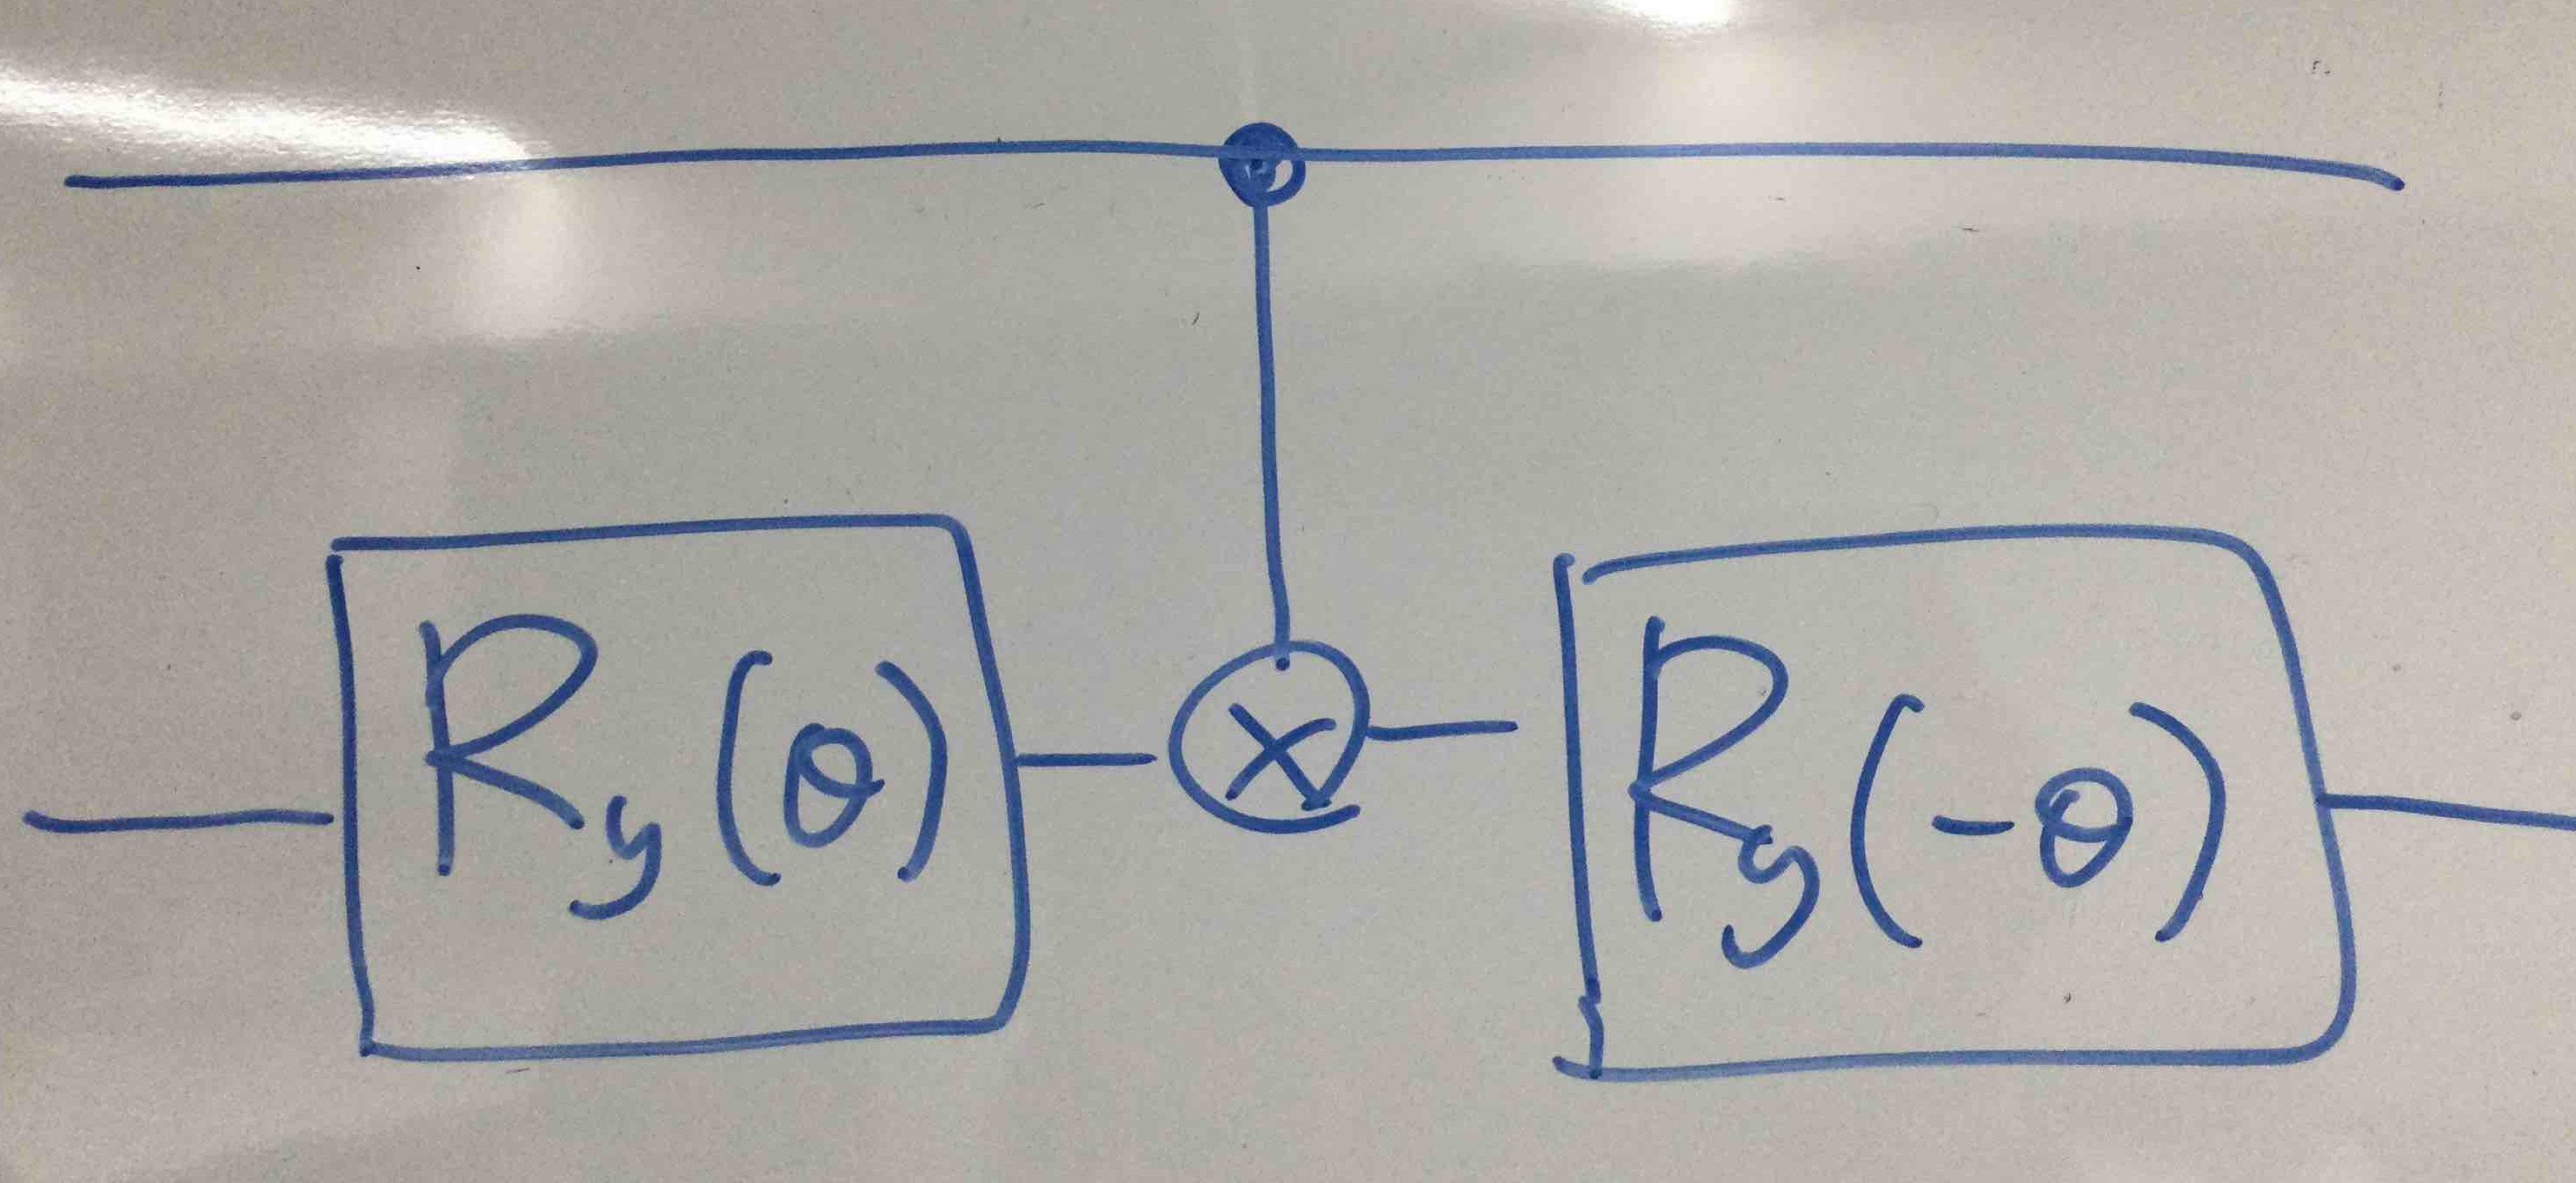
\includegraphics[width=0.5 \linewidth]{figs/fig_CFX_gate}
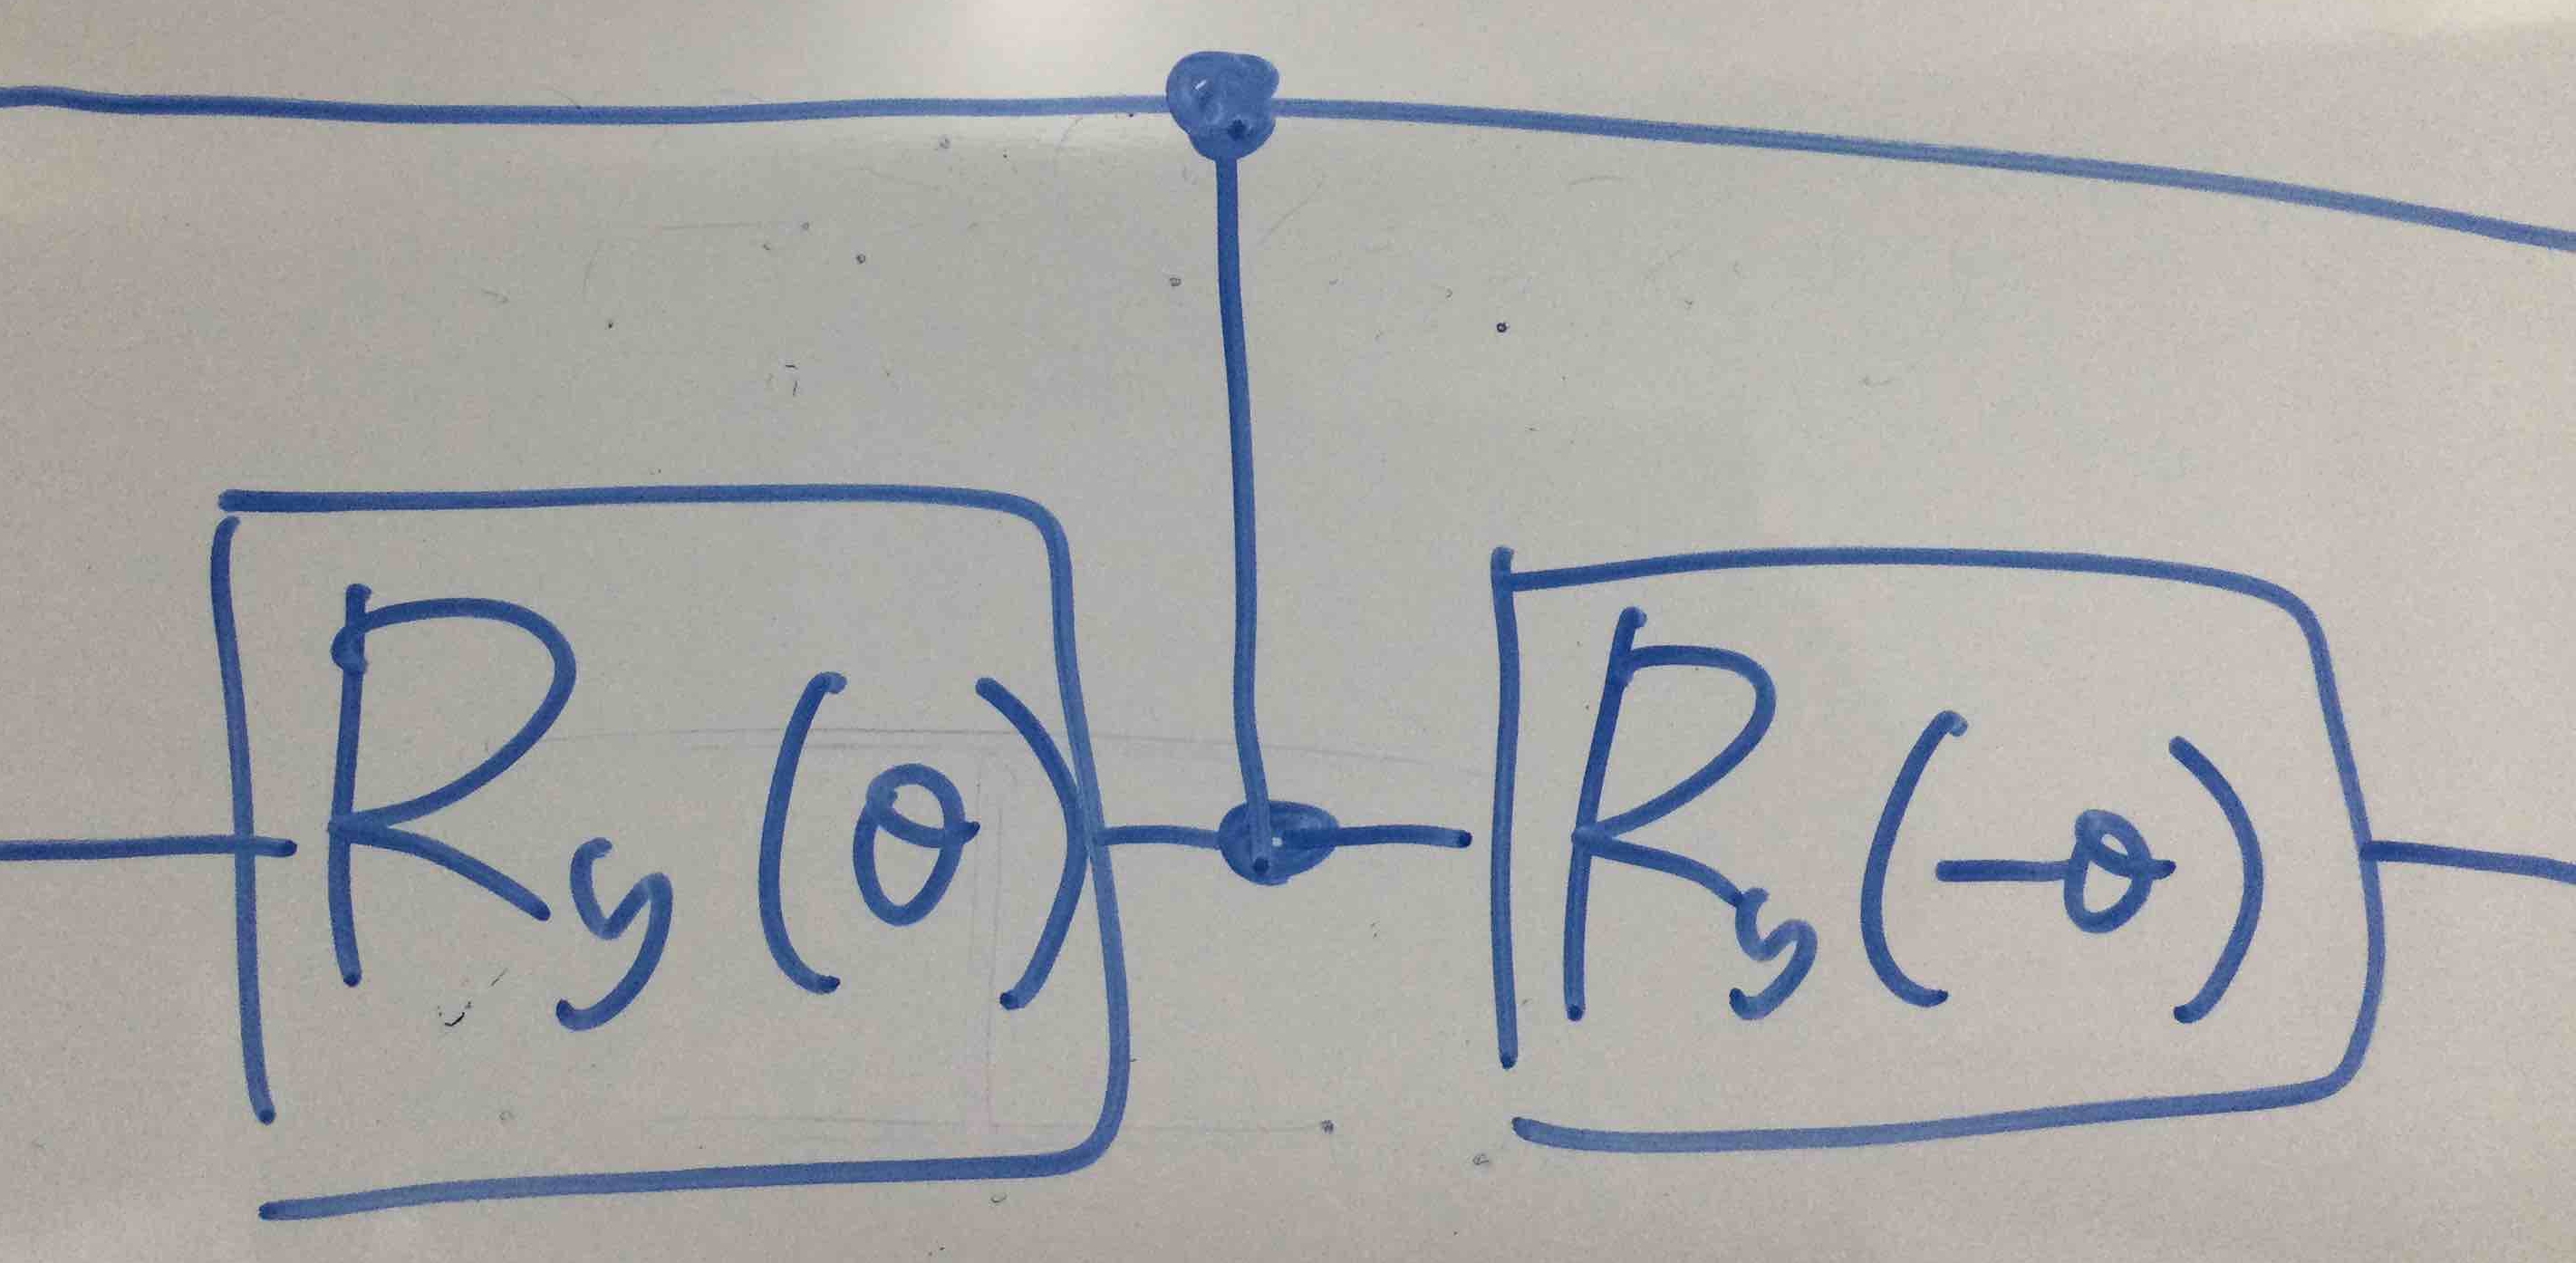
\includegraphics[width=0.5 \linewidth]{figs/fig_CFZ_gate}
\caption{Diagram of $CF^X_y$ gate (left) and $CF^Z_y$ gate (right)}
% \label{fig:cis}
\end{figure}

We also make use of $C^n(F^X_y)$ gate, which make use of $n-1$ ancilla qubits and $2 (n-1)$ Toffoli gates.
\begin{figure}
\centering
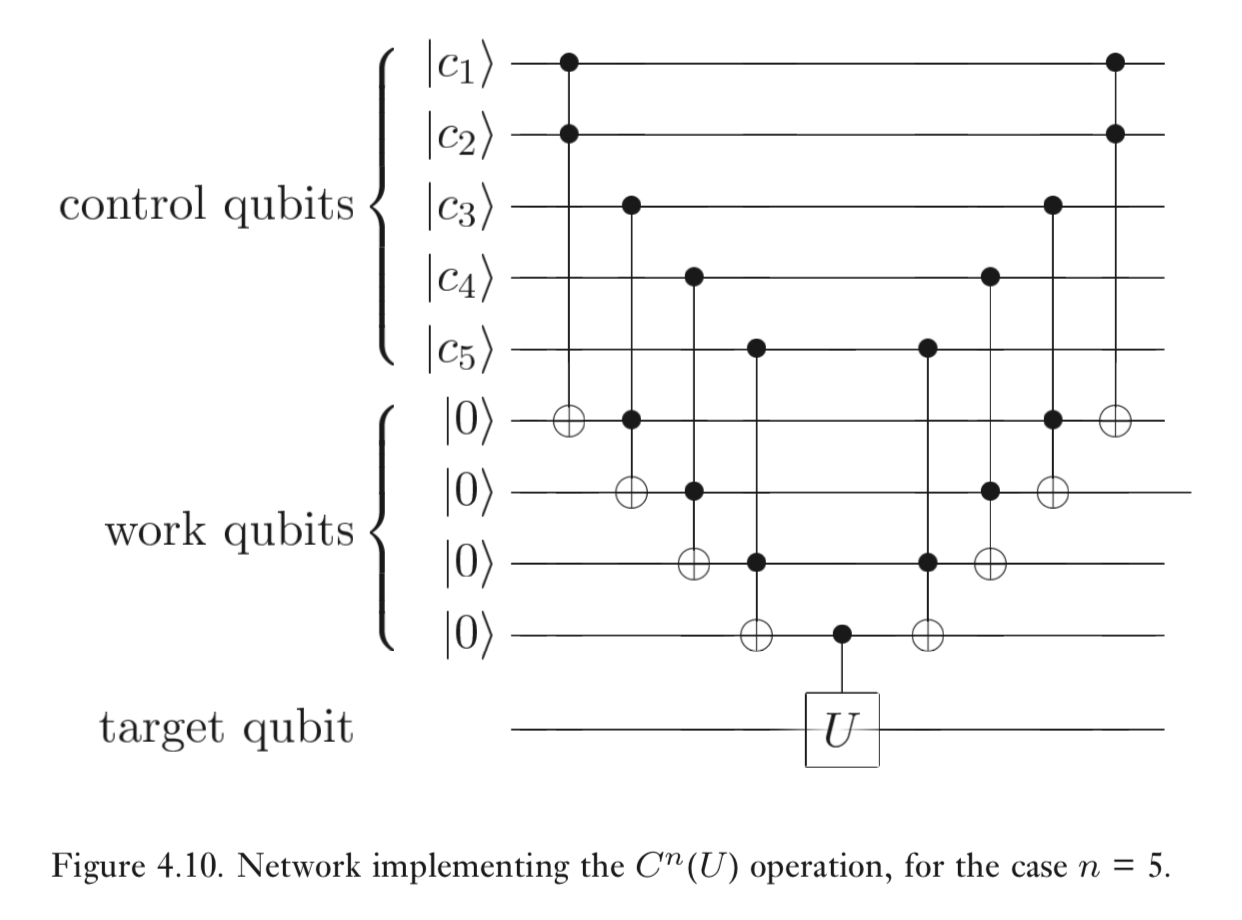
\includegraphics[width=0.5 \linewidth]{figs/fig_Cn_U_gate}
\caption{Implementation of $C^n (U)$ gate}
% \label{fig:cis}
\end{figure}

\subsubsection{Example of 4 spin-orbitals 2 electron state}
Consider the case where the number of spin-orbitals $n = 4$ and the number of electrons $m = 2$.
Applying the circuit shown in Fig on $\ket{0}^{\otimes 4}$ gives

\begin{figure}
\centering
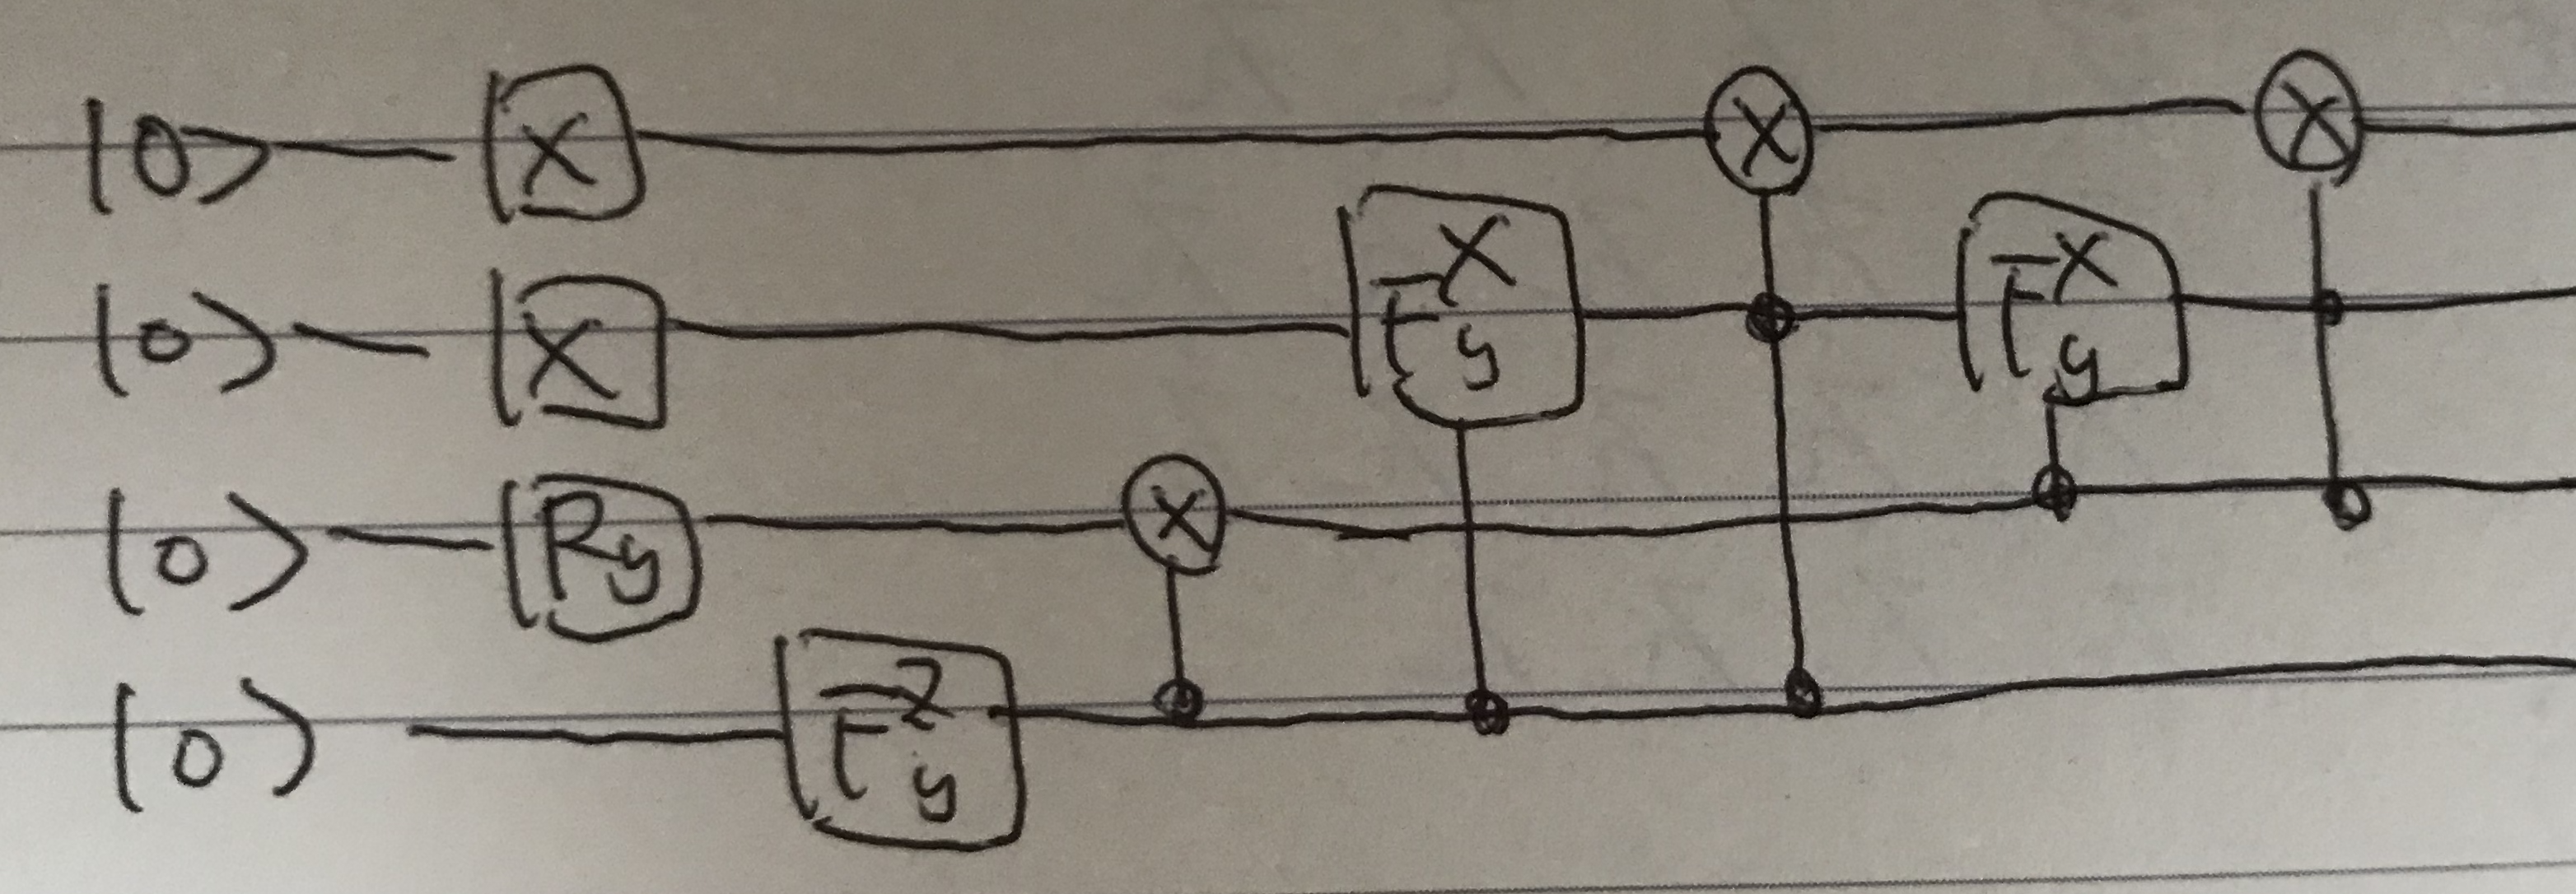
\includegraphics[width=0.75 \linewidth]{figs/fig_cis_circuit_2e_2o}
\caption{Implementation of circuit which generate CIS state for $(2e, 2o)$}
% \label{fig:cis}
\end{figure}

\begin{align*}
\ket{0}^{\otimes 4} 
&\xrightarrow{R_y(2 \theta_0) X_0 X_0} \cos(\theta_0) \ket{0011} + \sin(\theta_0) \ket{0111} \\
&\xrightarrow{CF^Z_y(\theta_1)} \cos(\theta_0) \ket{0011} + \sin(\theta_0) \left( \cos(\theta_1) \ket{0111} + \sin(\theta_1) \ket{1111} \right) \\
&\xrightarrow{\text{CNOT}_{32}} \cos(\theta_0) \ket{0011} + \sin(\theta_0) \left( \cos(\theta_1) \ket{0111} + \sin(\theta_1) \ket{1011} \right) \\
&\xrightarrow{CF^X_y(\theta_2)_{31}} 
\cos(\theta_0) \ket{0011} 
+ \sin(\theta_0) \cos(\theta_1) \ket{0111} 
+ \sin(\theta_0) \sin(\theta_1) (\cos(\theta_2) \ket{1001} + \sin(\theta_2) \ket{1011}) \\
&\xrightarrow{\text{Toffoli}_{310}} 
\cos(\theta_0) \ket{0011} 
+ \sin(\theta_0) \cos(\theta_1) \ket{0111} 
+ \sin(\theta_0) \sin(\theta_1) (\cos(\theta_2) \ket{1001} + \sin(\theta_2) \ket{1010}) \\
&\xrightarrow{CF^X_y(\theta_3)_{21}} 
\cos(\theta_0) \ket{0011} 
+ \sin(\theta_0) \cos(\theta_1) (\cos(\theta_3) \ket{0101} + \sin(\theta_3) \ket{0111})
+ \sin(\theta_0) \sin(\theta_1) (\cos(\theta_2) \ket{1001} + \sin(\theta_2) \ket{1010}) \\
&\xrightarrow{\text{Toffoli}_{210}}
\cos(\theta_0) \ket{0011} 
+ \sin(\theta_0) \cos(\theta_1) (\cos(\theta_3) \ket{0101} + \sin(\theta_3) \ket{0110}) \\
&+ \sin(\theta_0) \sin(\theta_1) (\cos(\theta_2) \ket{1001} + \sin(\theta_2) \ket{1010})
\end{align*}

\begin{equation}
\ket{\text{CIS}} 
= \alpha_0 \ket{0011} 
+ \alpha_1 \ket{1001}
+ \alpha_2 \ket{1010}
+ \alpha_3 \ket{0101} 
+ \alpha_4 \ket{0110} 
\end{equation}
where
\begin{align*}
\alpha_0 &= \cos(\theta_0) \\
\alpha_1 &= \sin(\theta_0) \sin(\theta_1) \cos(\theta_2) \\
\alpha_2 &= \sin(\theta_0) \sin(\theta_1) \sin(\theta_2) \\
\alpha_3 &= \sin(\theta_0) \cos(\theta_1) \cos(\theta_3) \\
\alpha_4 &= \sin(\theta_0) \cos(\theta_1) \sin(\theta_3)
\end{align*}

\subsubsection{Example of 8 spin-orbitals 4 electron state}
Consider the case where the number of spin-orbitals $n = 8$ and the number of electrons $m = 4$.
Applying the circuit shown in Fig on $\ket{0}^{\otimes 8}$ gives CIS state for such electron state.

\begin{figure}
\centering
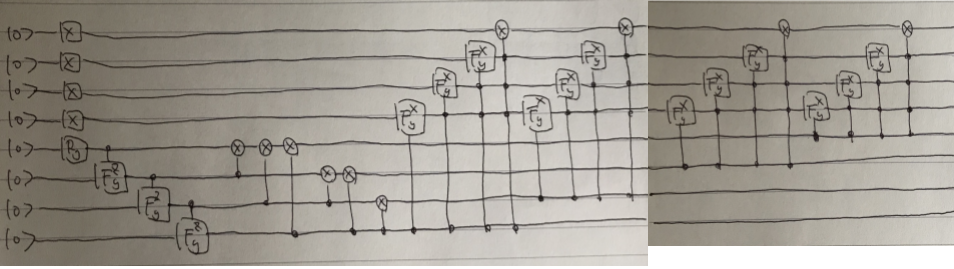
\includegraphics[width=0.75 \linewidth]{figs/fig_cis_circuit_4e_4o}
\caption{Implementation of circuit which generate CIS state for $(4e, 4o)$}
% \label{fig:cis}
\end{figure}

The circuit can be divided into six parts:
\begin{align*}
\ket{0}^{\otimes 8} 
&\xrightarrow{R_{y_4}(2 \theta_0) X_3 X_2 X_1 X_0} c_0 \ket{00001111} + s_0 \ket{00011111} \\
&\xrightarrow{CF^Z_y(\theta_1)} c_0 \ket{00001111} + s_0 (c_1 \ket{00011111} + s_1 \ket{00111111}) \\
&\xrightarrow{CF^Z_y(\theta_2)} 
c_0 \ket{00001111} 
+ s_0 c_1 \ket{00011111}
+ s_0 s_1 (c_2 \ket{00111111} + s_2 \ket{01111111} ) \\
&\xrightarrow{CF^Z_y(\theta_3)} 
c_0 \ket{00001111} 
+ s_0 c_1 \ket{00011111}
+ s_0 s_1 c_2 \ket{00111111}
+ s_0 s_1 s_2 (c_3 \ket{01111111} + s_3 \ket{11111111}) \\
& = \ket{\psi_1}
\end{align*}

\begin{align*}
\ket{\psi_1}
&\xrightarrow{\text{CNOT}_{74} \text{CNOT}_{64} \text{CNOT}_{54}} 
c_0 \ket{00001111} 
+ s_0 c_1 \ket{00011111}
+ s_0 s_1 c_2 \ket{00101111} \\
& \hspace{10em} + s_0 s_1 s_2 (c_3 \ket{01101111} + s_3 \ket{11101111}) \\
&\xrightarrow{\text{CNOT}_{65} \text{CNOT}_{75}} 
c_0 \ket{00001111} 
+ s_0 c_1 \ket{00011111}
+ s_0 s_1 c_2 \ket{00101111} \\
& \hspace{8em} + s_0 s_1 s_2 (c_3 \ket{01001111} + s_3 \ket{11001111}) \\
&\xrightarrow{\text{CNOT}_{76}} 
c_0 \ket{00001111} 
+ s_0 c_1 \ket{00011111}
+ s_0 s_1 c_2 \ket{00101111} + s_0 s_1 s_2 (c_3 \ket{01001111} + s_3 \ket{10001111}) \\
& = \ket{\psi_2} 
\end{align*}

\begin{align*}
\ket{\psi_2}
&\xrightarrow{CF^X_y(\theta_4)} 
c_0 \ket{00001111} 
+ s_0 c_1 \ket{00011111}
+ s_0 s_1 c_2 \ket{00101111}
+ s_0 s_1 s_2 c_3 \ket{01001111} \\
& \hspace{5em} + s_0 s_1 s_2 s_3 (c_4 \ket{10000111} + s_4 \ket{10001111}) \\
&\xrightarrow{C^2 F^X_y(\theta_5)} 
c_0 \ket{00001111} 
+ s_0 c_1 \ket{00011111}
+ s_0 s_1 c_2 \ket{00101111} 
+ s_0 s_1 s_2 c_3 \ket{01001111} \\
& \hspace{5em}  
+ s_0 s_1 s_2 s_3 c_4 \ket{10000111} 
+ s_0 s_1 s_2 s_3 s_4 (c_5 \ket{10001011} + s_5 \ket{10001111}) \\
&\xrightarrow{C^3 F^X_y(\theta_6)} 
c_0 \ket{00001111} 
+ s_0 c_1 \ket{00011111}
+ s_0 s_1 c_2 \ket{00101111}
+ s_0 s_1 s_2 c_3 \ket{01001111} \\
& \hspace{5em}
+ s_0 s_1 s_2 s_3 c_4 \ket{10000111}
+ s_0 s_1 s_2 s_3 s_4 c_5 \ket{10001011} \\
& \hspace{5em} 
+ s_0 s_1 s_2 s_3 s_4 s_5 (c_6 \ket{10001101} + s_6 \ket{10001111} ) \\
&\xrightarrow{\text{Toffoli}_{73210}} 
c_0 \ket{00001111} 
+ s_0 c_1 \ket{00011111}
+ s_0 s_1 c_2 \ket{00101111} 
+ s_0 s_1 s_1 c_3 \ket{01001111} \\
& \hspace{5em} 
+ s_0 s_1 s_2 s_3 c_4 \ket{10000111}
+ s_0 s_1 s_2 s_3 s_4 c_5 \ket{10001011} \\
& \hspace{5em} 
+ s_0 s_1 s_2 s_3 s_4 s_5 (c_6 \ket{10001101} + s_6 \ket{10001110} ) \\
& = \ket{\psi_3} 
\end{align*}

\begin{align*}
\ket{\psi_3}
&\xrightarrow{CF^X_y(\theta_7)} 
c_0 \ket{00001111} 
+ s_0 c_1 \ket{00011111}
+ s_0 s_1 c_2 \ket{00101111} 
+ s_0 s_1 s_2 c_3 (c_7 \ket{01000111} + s_7 \ket{01001111}) \\
& \hspace{5em} 
+ s_0 s_1 s_2 s_3 c_4 \ket{10000111}
+ s_0 s_1 s_2 s_3 s_4 c_5 \ket{10001011} \\
& \hspace{5em} 
+ s_0 s_1 s_2 s_3 s_4 s_5 (c_6 \ket{10001101} + s_6 \ket{10001110} ) \\
&\xrightarrow{C^2 F^X_y(\theta_8)} 
c_0 \ket{00001111} 
+ s_0 c_1 \ket{00011111}
+ s_0 s_1 c_2 \ket{00101111} 
+ s_0 s_1 s_2 c_3 c_7 \ket{01000111} \\
& \hspace{5em} 
+ s_0 s_1 s_2 c_3 s_7 (c_8 \ket{01001011} + s_8 \ket{01001111}) 
+ s_0 s_1 s_2 s_3 c_4 \ket{10000111} \\
& \hspace{5em} 
+ s_0 s_1 s_2 s_3 s_4 c_5 \ket{10001011}
+ s_0 s_1 s_2 s_3 s_4 s_5 (c_6 \ket{10001101} + s_6 \ket{10001110} ) \\
&\xrightarrow{C^3 F^X_y(\theta_9)} 
c_0 \ket{00001111} 
+ s_0 c_1 \ket{00011111}
+ s_0 s_1 c_2 \ket{00101111} 
+ s_0 s_1 s_2 c_3 c_7 \ket{01000111} \\
& \hspace{5em} 
+ s_0 s_1 s_2 c_3 s_7 c_8 \ket{01001011}
+ s_0 s_1 s_2 c_3 s_7 s_8 (c_9 \ket{01001101} + s_9 \ket{01001111}) \\
& \hspace{5em} 
+ s_0 s_1 s_2 s_3 c_4 \ket{10000111}
+ s_0 s_1 s_2 s_3 s_4 c_5 \ket{10001011} \\
& \hspace{5em} 
+ s_0 s_1 s_2 s_3 s_4 s_5 (c_6 \ket{10001101} + s_6 \ket{10001110} ) \\
&\xrightarrow{\text{Toffoli}_{63210}} 
c_0 \ket{00001111} 
+ s_0 c_1 \ket{00011111}
+ s_0 s_1 c_2 \ket{00101111} 
+ s_0 s_1 s_2 c_3 c_7 \ket{01000111} \\
& \hspace{5em} 
+ s_0 s_1 s_2 c_3 s_7 c_8 \ket{01001011}
+ s_0 s_1 s_2 c_3 s_7 s_8 (c_9 \ket{01001101} + s_9 \ket{01001110}) \\
& \hspace{5em} 
+ s_0 s_1 s_2 s_3 c_4 \ket{10000111}
+ s_0 s_1 s_2 s_3 s_4 c_5 \ket{10001011} \\
& \hspace{5em} 
+ s_0 s_1 s_2 s_3 s_4 s_5 (c_6 \ket{10001101} + s_6 \ket{10001110} ) \\
& = \ket{\psi_4} 
\end{align*}

\begin{align*}
\ket{\psi_4}
&\xrightarrow{CF^X_y(\theta_{10})} 
c_0 \ket{00001111} 
+ s_0 c_1 \ket{00011111}
+ s_0 s_1 c_2 (c_{10} \ket{00100111} + s_{10} \ket{00101111}) \\
& \hspace{5em} 
+ s_0 s_1 s_2 c_3 c_7 \ket{01000111}
+ s_0 s_1 s_2 c_3 s_7 c_8 \ket{01001011} \\
& \hspace{5em} 
+ s_0 s_1 s_2 c_3 s_7 s_8 (c_9 \ket{01001101} + s_9 \ket{01001110}) \\
& \hspace{5em} 
+ s_0 s_1 s_2 s_3 c_4 \ket{10000111}
+ s_0 s_1 s_2 s_3 s_4 c_5 \ket{10001011} \\
& \hspace{5em} 
+ s_0 s_1 s_2 s_3 s_4 s_5 (c_6 \ket{10001101} + s_6 \ket{10001110} ) \\
&\xrightarrow{C^2 F^X_y(\theta_{11})} 
c_0 \ket{00001111} 
+ s_0 c_1 \ket{00011111}
+ s_0 s_1 c_2 c_{10} \ket{00100111} \\
& \hspace{5em} 
+ s_0 s_1 c_2 s_{10} (c_{11} \ket{00101011} + s_{11} \ket{00101111}) \\
& \hspace{5em} 
+ s_0 s_1 s_2 c_3 c_7 \ket{01000111}
+ s_0 s_1 s_2 c_3 s_7 c_8 \ket{01001011} \\
& \hspace{5em} 
+ s_0 s_1 s_2 c_3 s_7 s_8 (c_9 \ket{01001101} + s_9 \ket{01001110}) \\
& \hspace{5em} 
+ s_0 s_1 s_2 s_3 c_4 \ket{10000111}
+ s_0 s_1 s_2 s_3 s_4 c_5 \ket{10001011} \\
& \hspace{5em} 
+ s_0 s_1 s_2 s_3 s_4 s_5 (c_6 \ket{10001101} + s_6 \ket{10001110} ) \\
&\xrightarrow{C^3 F^X_y(\theta_{12})} 
c_0 \ket{00001111} 
+ s_0 c_1 \ket{00011111}
+ s_0 s_1 c_2 c_{10} \ket{00100111}
+ s_0 s_1 c_2 s_{10} c_{11} \ket{00101011} \\
& \hspace{5em} 
+ s_0 s_1 c_2 s_{10} s_{11} (c_{12} \ket{00101101} + s_{12} \ket{00101111}) \\
& \hspace{5em} 
+ s_0 s_1 s_2 c_3 c_7 \ket{01000111}
+ s_0 s_1 s_2 c_3 s_7 c_8 \ket{01001011} \\
& \hspace{5em} 
+ s_0 s_1 s_2 c_3 s_7 s_8 (c_9 \ket{01001101} + s_9 \ket{01001110}) \\
& \hspace{5em} 
+ s_0 s_1 s_2 s_3 c_4 \ket{10000111}
+ s_0 s_1 s_2 s_3 s_4 c_5 \ket{10001011} \\
& \hspace{5em} 
+ s_0 s_1 s_2 s_3 s_4 s_5 (c_6 \ket{10001101} + s_6 \ket{10001110} ) \\
&\xrightarrow{\text{Toffoli}_{53210}} 
c_0 \ket{00001111} 
+ s_0 c_1 \ket{00011111}
+ s_0 s_1 c_2 c_{10} \ket{00100111}
+ s_0 s_1 c_2 s_{10} c_{11} \ket{00101011} \\
& \hspace{5em} 
+ s_0 s_1 c_2 s_{10} s_{11} (c_{12} \ket{00101101} + s_{12} \ket{00101110}) \\
& \hspace{5em} 
+ s_0 s_1 s_2 c_3 c_7 \ket{01000111}
+ s_0 s_1 s_2 c_3 s_7 c_8 \ket{01001011} \\
& \hspace{5em} 
+ s_0 s_1 s_2 c_3 s_7 s_8 (c_9 \ket{01001101} + s_9 \ket{01001110}) \\
& \hspace{5em} 
+ s_0 s_1 s_2 s_3 c_4 \ket{10000111}
+ s_0 s_1 s_2 s_3 s_4 c_5 \ket{10001011} \\
& \hspace{5em} 
+ s_0 s_1 s_2 s_3 s_4 s_5 (c_6 \ket{10001101} + s_6 \ket{10001110} ) \\
& = \ket{\psi_5} 
\end{align*}

\begin{align*}
\ket{\psi_5}
&\xrightarrow{CF^X_y(\theta_{13})} 
c_0 \ket{00001111} 
+ s_0 c_1 (c_{13} \ket{00010111} + s_{13} \ket{00011111})
+ s_0 s_1 c_2 c_{10} \ket{00100111} \\
& \hspace{5em} 
+ s_0 s_1 c_2 s_{10} c_{11} \ket{00101011}
+ s_0 s_1 c_2 s_{10} s_{11} (c_{12} \ket{00101101} + s_{12} \ket{00101110}) \\
& \hspace{5em} 
+ s_0 s_1 s_2 c_3 c_7 \ket{01000111}
+ s_0 s_1 s_2 c_3 s_7 c_8 \ket{01001011} \\
& \hspace{5em} 
+ s_0 s_1 s_2 c_3 s_7 s_8 (c_9 \ket{01001101} + s_9 \ket{01001110}) \\
& \hspace{5em} 
+ s_0 s_1 s_2 s_3 c_4 \ket{10000111}
+ s_0 s_1 s_2 s_3 s_4 c_5 \ket{10001011} \\
& \hspace{5em} 
+ s_0 s_1 s_2 s_3 s_4 s_5 (c_6 \ket{10001101} + s_6 \ket{10001110} ) \\
&\xrightarrow{C^2 F^X_y(\theta_{14})} 
c_0 \ket{00001111} 
+ s_0 c_1 c_{13} \ket{00010111}
+ s_0 c_1 s_{13} (c_{14} \ket{00011011} + s_{14} \ket{00011111}) \\
& \hspace{5em} 
+ s_0 s_1 c_2 c_{10} \ket{00100111} 
+ s_0 s_1 c_2 s_{10} c_{11} \ket{00101011} \\
& \hspace{5em} 
+ s_0 s_1 c_2 s_{10} s_{11} (c_{12} \ket{00101101} + s_{12} \ket{00101110}) \\
& \hspace{5em} 
+ s_0 s_1 s_2 c_3 c_7 \ket{01000111}
+ s_0 s_1 s_2 c_3 s_7 c_8 \ket{01001011} \\
& \hspace{5em} 
+ s_0 s_1 s_2 c_3 s_7 s_8 (c_9 \ket{01001101} + s_9 \ket{01001110}) \\
& \hspace{5em} 
+ s_0 s_1 s_2 s_3 c_4 \ket{10000111}
+ s_0 s_1 s_2 s_3 s_4 c_5 \ket{10001011} \\
& \hspace{5em} 
+ s_0 s_1 s_2 s_3 s_4 s_5 (c_6 \ket{10001101} + s_6 \ket{10001110} ) \\
&\xrightarrow{C^3 F^X_y(\theta_{15})} 
c_0 \ket{00001111} 
+ s_0 c_1 c_{13} \ket{00010111}
+ s_0 c_1 s_{13} c_{14} \ket{00011011} \\
& \hspace{5em} 
+ s_0 c_1 s_{13} s_{14} (c_{15} \ket{00011101} + s_{15} \ket{00011111}) \\
& \hspace{5em} 
+ s_0 s_1 c_2 c_{10} \ket{00100111} 
+ s_0 s_1 c_2 s_{10} c_{11} \ket{00101011} \\
& \hspace{5em} 
+ s_0 s_1 c_2 s_{10} s_{11} (c_{12} \ket{00101101} + s_{12} \ket{00101110}) \\
& \hspace{5em} 
+ s_0 s_1 s_2 c_3 c_7 \ket{01000111}
+ s_0 s_1 s_2 c_3 s_7 c_8 \ket{01001011} \\
& \hspace{5em} 
+ s_0 s_1 s_2 c_3 s_7 s_8 (c_9 \ket{01001101} + s_9 \ket{01001110}) \\
& \hspace{5em} 
+ s_0 s_1 s_2 s_3 c_4 \ket{10000111}
+ s_0 s_1 s_2 s_3 s_4 c_5 \ket{10001011} \\
& \hspace{5em} 
+ s_0 s_1 s_2 s_3 s_4 s_5 (c_6 \ket{10001101} + s_6 \ket{10001110} ) \\
&\xrightarrow{\text{Toffoli}_{43210}} 
c_0 \ket{00001111} 
+ s_0 c_1 c_{13} \ket{00010111}
+ s_0 c_1 s_{13} c_{14} \ket{00011011} \\
& \hspace{5em} 
+ s_0 c_1 s_{13} s_{14} (c_{15} \ket{00011101} + s_{15} \ket{00011110}) \\
& \hspace{5em} 
+ s_0 s_1 c_2 c_{10} \ket{00100111} 
+ s_0 s_1 c_2 s_{10} c_{11} \ket{00101011} \\
& \hspace{5em} 
+ s_0 s_1 c_2 s_{10} s_{11} (c_{12} \ket{00101101} + s_{12} \ket{00101110}) \\
& \hspace{5em} 
+ s_0 s_1 s_2 c_3 c_7 \ket{01000111}
+ s_0 s_1 s_2 c_3 s_7 c_8 \ket{01001011} \\
& \hspace{5em} 
+ s_0 s_1 s_2 c_3 s_7 s_8 (c_9 \ket{01001101} + s_9 \ket{01001110}) \\
& \hspace{5em} 
+ s_0 s_1 s_2 s_3 c_4 \ket{10000111}
+ s_0 s_1 s_2 s_3 s_4 c_5 \ket{10001011} \\
& \hspace{5em} 
+ s_0 s_1 s_2 s_3 s_4 s_5 (c_6 \ket{10001101} + s_6 \ket{10001110} ) \\
\end{align*}

Here we denote $c_i = \cos(\theta_i)$ and $s_i = \sin(\theta_i)$, 
and $\text{Toffoli}_{c_1 c_2 \cdots c_n t}$ as generalized Toffoli gate which has $n$ control qubits $c_1 c_2 \cdots c_n$.

We see that we obtain

\begin{align*}
\ket{\text{CIS}} 
&= \alpha_0 \ket{00001111} 
+ \alpha_1 \ket{00011110} 
+ \alpha_2 \ket{00101110} 
+ \alpha_3 \ket{01001110}
+ \alpha_4 \ket{10001110} \\
&+ \alpha_5 \ket{00011101} 
+ \alpha_6 \ket{00101101} 
+ \alpha_7 \ket{01001101} 
+ \alpha_8 \ket{10001101} \\
&+ \alpha_9 \ket{00011011} 
+ \alpha_{10} \ket{00101011}
+ \alpha_{11} \ket{01001011}
+ \alpha_{12} \ket{10001011} \\
&+ \alpha_{13} \ket{00010111} 
+ \alpha_{14} \ket{00100111}
+ \alpha_{15} \ket{01000111}
+ \alpha_{16} \ket{10000111},
\end{align*}
where
\begin{align*}
\alpha_0 &= c_0 \\
\alpha_1 &= s_0 c_1 s_{13} s_{14} s_{15} \\
\alpha_2 &= s_0 s_1 c_2 s_{10} s_{11} s_{12} \\
\alpha_3 &= s_0 s_1 s_2 c_3 s_7 s_8 s_9 \\
\alpha_4 &= s_0 s_1 s_2 s_3 s_4 s_5 s_6 \\
\alpha_5 &= s_0 c_1 s_{13} s_{14} c_{15} \\
\alpha_6 &= s_0 s_1 c_2 s_{10} s_{11} c_{12} \\
\alpha_7 &= s_0 s_1 s_2 c_3 s_7 s_8 c_9 \\
\alpha_8 &= s_0 s_1 s_2 s_3 s_4 s_5 c_6 \\
\alpha_9 &= s_0 c_1 s_{13} c_{14} \\ 
\alpha_{10} &= s_0 s_1 c_2 s_{10} c_{11} \\
\alpha_{11} &= s_0 s_1 s_2 c_3 s_7 c_8 \\
\alpha_{12} &= s_0 s_1 s_2 s_3 s_4 c_5 \\
\alpha_{13} &= s_0 c_1 c_{13} \\
\alpha_{14} &= s_0 s_1 c_2 c_{10} \\
\alpha_{15} &= s_0 s_1 s_2 c_3 c_7 \\
\alpha_{16} &= s_0 s_1 s_2 s_3 c_4 
\end{align*}


\subsubsection{Resource estimation for general cases}
Consider the case where the number of qubits $n$ and the number of electrons $m$.
As can be seen from the above examples, we need 
$m$ $X$-gates, 
one $R_y$-gate, 
$(n-m-1)$ $CF^Z_y$ gates, 
$(n-m-1) (n-m) / 2$ CNOT gates,
$(n-m)$ $CF^X_y, C^2 F^X_y, \cdots C^{m-1} F^X_y$ gates, and 
$(n-m)$ $\text{Toffoli}_{c_1 c_2 \cdots c_m t}$ gates.
Note that each $C^{m-1} F^X_y$ gate consists of $m-1$ ancilla qubits, $2(m-1)$ Toffoli gates and one $CF^X_y$ gate, and
each $(n-m)$ $\text{Toffoli}_{c_1 c_2 \cdots c_m t}$ gate consists of $m-2$ ancilla qubits, $(2m-1)$ Toffoli gates.
\end{document}  